\documentclass[11pt,a4paper]{report}
\usepackage[utf8x]{inputenc}
\usepackage[italian]{babel}
\usepackage{amsmath}
\usepackage{amsfonts}
\usepackage{float}
\usepackage{amssymb}
\usepackage{afterpage}
\usepackage{xcolor}
\usepackage{graphicx}

\usepackage{listings}
%% listings-modelica.cfg
%% Copyright 2014 Martin Sjoelund, Dietmar Winkler
%
% This work may be distributed and/or modified under the
% conditions of the LaTeX Project Public License, either version 1.3
% of this license or (at your option) any later version.
% The latest version of this license is in
%   http://www.latex-project.org/lppl.txt
% and version 1.3 or later is part of all distributions of LaTeX
% version 2005/12/01 or later.
%
% This work has the LPPL maintenance status `maintained'.
%
% The Current Maintainer of this work is Dietmar Winkler
%
% Code repository https://github.com/modelica-tools/listings-modelica
%
% This work consists of the file listings-modelica.cfg

\lstdefinelanguage{modelica}
{
  morekeywords=[1]{
    algorithm,and,annotation,as,assert,block,break,case,class,connect,connector,
    constant,constrainedby,der,discrete,each,else,elseif,elsewhen,encapsulated,
    end,enumeration,equality,equation,expandable,extends,external,failure,final,
    flow,for,function,guard,if,import,in,initial,inner,input,List,local,loop,
    match,matchcontinue,model,not,operator,Option,or,outer,output,package,parameter,
    partial,protected,public,record,Real,redeclare,replaceable,return,stream,
    subtypeof,then,Tuple,type,uniontype,when,while},
  morekeywords=[2]{true, false},
  % Do not make true,false keywords because fn(true,x, false ) shows up as fn(true,x, *false*)
  morekeywords=[3]{optimization,constraint}, % Optimica keywords
  morekeywords=[4]{objective,startTime,finalTime,initialGuess},
  sensitive=true,
  comment=[l]//,
  morecomment=[s]{/*}{*/},
  alsodigit={.,-},
  morestring=[b]',
  morestring=[b]",
}[keywords,comments,strings]

\definecolor{keywordcolor1}{rgb}{0,0,.4}
\definecolor{keywordcolor2}{rgb}{.90,0,0}
\definecolor{keywordcolor3}{rgb}{.4,0,.8}
\definecolor{keywordcolor4}{rgb}{0.5,0,0.5}
\definecolor{stringcolor}{rgb}{0.133,0.545,0.133}
% \definecolor{listingbgcolor}{rgb}{0.95,0.95,0.95}

\lstset{
  breaklines=true,
  language=modelica,
  basicstyle=\ttfamily,
  keywordstyle=[1]\color{keywordcolor1}\bfseries,
  keywordstyle=[2]\color{keywordcolor2},
  keywordstyle=[3]\color{keywordcolor3}\bfseries,
  keywordstyle=[4]\color{keywordcolor4},
  stringstyle=\color{stringcolor},
%  backgroundcolor=\color{listingbgcolor},
  framexleftmargin=5pt,
  xleftmargin=5pt,
  xrightmargin=5pt,
  showstringspaces=false
}

\newcommand{\code}[1]{\lstinline|#1|}
\newcommand{\modelica}[1]{\lstinline[language=modelica]|#1|}

\lstset{
	numbers=left, 
	numberstyle=\small,
	numbersep=8pt, 
	frame=single, 
	language=Modelica,
	framexleftmargin=15pt,
	basicstyle=\footnotesize\ttfamily,
	keywordstyle=\color{purple},
	numberstyle=\tiny\color{gray}
}

\newcommand{\modelicaclass}[1]{
	\lstinputlisting[firstline=9]{../Implementazioni algoritmo/openmodelica/classes/#1}
}

\newcommand{\emptypage}[0]{\afterpage{\null\newpage}}

\newcommand{\name}[1]{{\ttfamily #1}}

\graphicspath{ {./images/} }
\author{Gianluca Mondini}
\title{Tesi (titolo da definire)}

\begin{document}

\setlength{\parindent}{0pt}

%TODO sistemare i pagebreak, in particolare quelli tra capitoli
%TODO controllare che i codici non vengano spezzati tra più pagine, e nel caso usare \begin{figure} .. se necessario
%TODO scegliere un tempo verbale e tenerlo costante per tutto il documento
%TODO controllare i "punti" di fine frase

%\maketitle

%\pagebreak

\emptypage

\chapter*{Prefazione}

%TODO scrivere alla fine

{\em \large
L'obiettivo di questa trattazione è di illustrare l'implementazione di un insieme di classi OpenModelica con lo scopo di controllare un insieme di droni, per permettere ad esso di disporsi in modo equo su una data superficie.

In particolare, si vedrà l'implementazione dell'algoritmo di Lloyd.

È prevista la realizzazione di un modulo nell'ambiente OpenModelica che permetta di simulare il suddetto algoritmo; più avanti verranno illustrate parti di codice e verranno fornite informazioni relative alla sua implementazione.
}
\pagebreak

\emptypage

\tableofcontents

\pagebreak

%\chapter*{Parole chiave}

%Prima di procedere con la trattazione, è necessario indicare alcune parole chiave presenti in questo documento e nel codice dell'implementazione

%\begin{description}
%	\item[Drone] Velivolo che, nel nostro caso di interesse, è rappresentato come un punto bidimensionale
%	\item[Area] Poligono convesso che delimita l'algoritmo;
%	\item[Cella] Porzione di spazio alla quale appartiene un drone; la cella relativa ad un drone è l'insieme di punti dell'area per i quali, tra tutti i vari droni, quello appartenente alla cella è il più vicino
%\end{description}

%\pagebreak

\emptypage

\chapter{Il drone e i suoi componenti}

\begin{figure}[H]
\centering
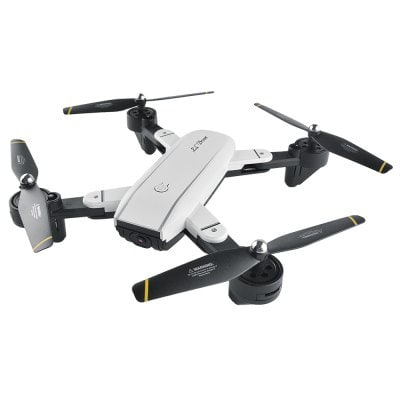
\includegraphics[scale=0.5]{drone.jpg}
\end{figure}

Possiamo schematizzare, ai fini di questa trattazione, un \textit{drone} mediante tre componenti: il \textit{centro fisico}, il \textit{controllo di volo} e il \textit{controllo della traiettoria}.

%TODO rivedere i nomi delle 3 componenti

%TODO inserire qui uno schemino che mostri i 3 componenti connessi tra loro

\paragraph{Centro fisico}

Il centro fisico è un'astrazione che rappresenta il rapporto del drone con il mondo esterno. Vengono qui considerati parametri come la massa, la velocità, l'accelerazione, la posizione, la rotazione, la velocità di rotazione dei motori e la potenza ad essi fornita.

\paragraph{Controllo di volo}

Il centro di volo considera il drone come un velivolo, e utilizzando i dati forniti dal centro fisico e dal controllo della traiettoria permette il controllo della direzione, della quota e della velocità.

\paragraph{Controllo della traiettoria}

Componente centrale della trattazione, il controllo della traiettoria ha la funzione di comunicare al centro di volo la posizione da raggiungere.

\

Nel nostro modello astratto, il controllo della traiettoria si orienta utilizzando la funzione \name{TargetPos}, la cui ideazione e implementazione viene illustrata in seguito.

\section{Ipotesi e semplificazioni}

%TODO

La trattazione e l'implementazione richiedono che vengano effettuate alcune ipotesi semplificative in relazione al mondo esterno nel quale l'algoritmo andrà ad operare. In particolare, si suppone che:

\begin{itemize}
	\item l'area nella quale il drone opera sia un poligono convesso
	\item non siano presenti degli ostacoli all'interno dell'area, in quanto questi non verrebbero considerati dal controllo di traiettoria portando il drone a una collisione
	\item il mondo nel quale il drone opera sia bidimensionale, ovvero si suppone che non sia definita una terza componente $z$ per le tuple rappresentanti la posizione. Nell'implementazione pratica, quest'ipotesi può essere gestita mediante l'utilizzo di un valore costante per la coordinata $z$ (ad esempio ogni drone si trova a 650 m sul livello del mare) oppure tale coordinata può essere determinata in funzione della distanza dal suolo.
\end{itemize}

La trattazione della funzione \name{TargetPos} richiede la conoscenza di aspetti teorici legati all'algoritmo di Lloyd.

\chapter{Diagramma di Voronoi}

TODO: questo l'ho preso da Wikipedia, riscriverlo.

In matematica, un diagramma di Voronoi (dal nome di Georgij Voronoi), anche detto tassellatura, partizione o decomposizione di Voronoi, o tassellatura di Dirichlet (dal nome di Lejeune Dirichlet) è un particolare tipo di decomposizione di uno spazio metrico determinata dalle distanze rispetto ad un determinato insieme discreto di elementi dello spazio (ad esempio, un insieme finito di punti).

Nel caso più semplice e comune, quello del piano, dato un insieme finito di punti S, il diagramma di Voronoi per S è la partizione del piano che associa una regione V(p) ad ogni punto p in S in modo tale che tutti i punti all'interno del perimetro di V(p) siano più vicini a p che a ogni altro punto in S.

TODO: spiegare cos'è la tassellazione di voronoi centroidale

\chapter{L'algoritmo di Lloyd}

L'algoritmo di Lloyd, conosciuto anche con il nome di \textit{iterazione di Voronoi}, è un algoritmo che permette di suddividere un'area in celle convesse uniformemente dimensionate. 

\

Tale suddivisione è denominata \textit{tassellazione di Voronoi centroidale}, ed è spesso indicata con la sigla \textit{CVT} (dall'inglese \textit{Centroidal Voronoi Tesselation}).

\begin{figure}[H]
\centering
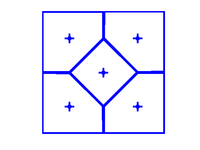
\includegraphics[width=4.5cm]{cvt1.png}
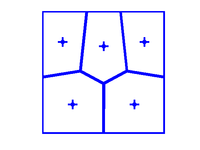
\includegraphics[width=4.5cm]{cvt2.png}
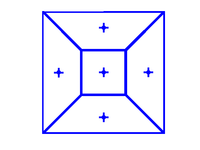
\includegraphics[width=4.5cm]{cvt3.png}
\caption{Tre esempi di CVT a 5 punti su un area quadrata}
\end{figure}

% L'algoritmo, che prende il nome da Stuart P. Lloyd, il suo ideatore, è implementato mediante iterazioni continue dell'algoritmo di Voronoi.

L'algoritmo, che prende il nome da Stuart P. Lloyd, il suo ideatore, è implementato mediante iterazioni continue dell'algoritmo di Voronoi.

In natura sono riscontrabili diversi esempi di CVT, come la struttura macroscopica del \textit{selciato del gigante} oppure le celle della cornea dell'occhio umano.

\begin{figure}[H]
\centering
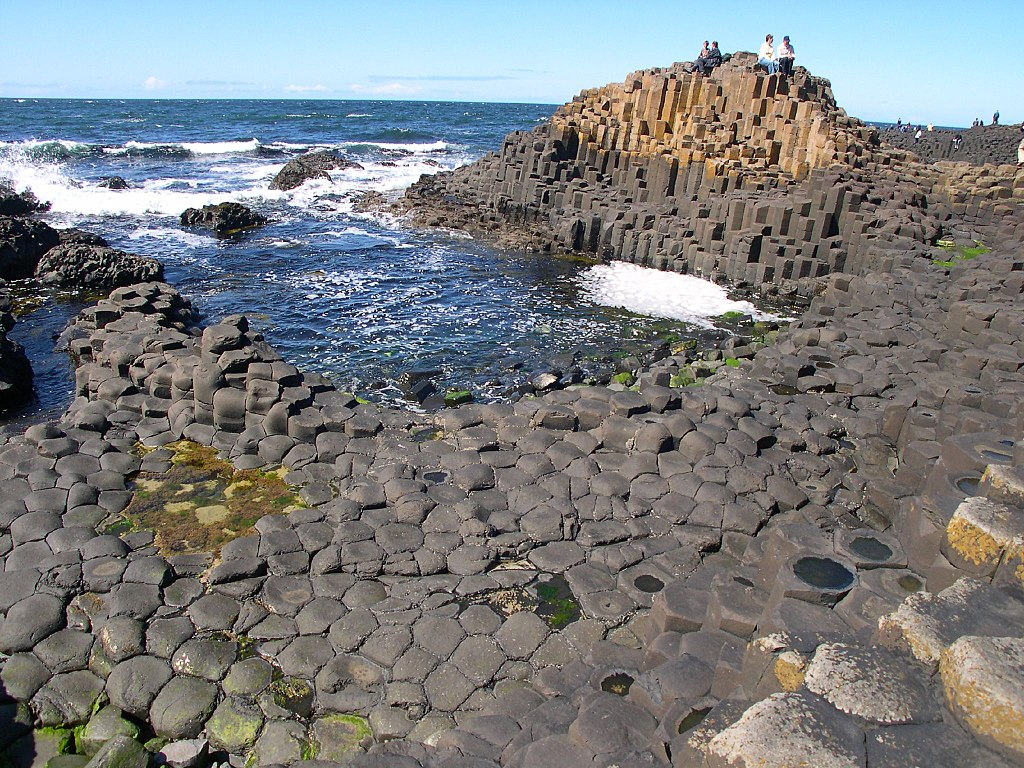
\includegraphics[width=14cm]{selciato_del_gigante.jpg}
\caption{Scala del gigante, Irlanda del Nord}
\end{figure}

\section{Descrizione dell'algoritmo (TODO)}

L'algoritmo esegue ripetutamente i seguenti passi:

\begin{enumerate}
	\item Viene generato il diagramma di Voronoi
	\item Per ogni cella trovata, viene determinato il \textit{baricentro}
	\item Ogni punto viene spostato in corrispondenza del \textit{baricentro} della propria \textit{cella di Voronoi}
\end{enumerate}

\section{Esempio di applicazione dell'algoritmo}

Viene qui presentata l'applicazione dell'algoritmo di Lloyd ad un'area quadrata nella quale sono presenti 5 partizioni.

Le croci rappresentano i \textit{baricentri} delle varie partizioni; i punti rossi sono i droni, e le linee nere delimitano le varie celle dei singoli droni. Il quadrato che racchiude il tutto è l'area entro la quale i droni devono equidisporsi.

\paragraph{Iterazione 1}

I droni sono mediamente distanti dal centro di massa della propria cella.

\begin{figure}[H]
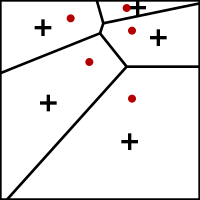
\includegraphics[width=5cm]{lloyd_iterazione_1.png}
\centering
\end{figure}

\paragraph{Iterazione 2}

La distanza media tra i droni e il centro di massa delle rispettive celle è ridotta. Si noti come si è modificata la forma delle varie celle, in conseguenza del movimento dei vari droni.

\begin{figure}[H]
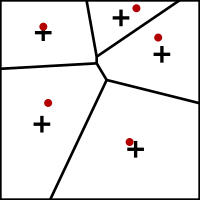
\includegraphics[width=5cm]{lloyd_iterazione_2.png}
\centering
\end{figure}

\paragraph{Iterazione 3}

La distanza media tra i droni ed il centro di massa è quasi nulla. L'algoritmo è prossimo alla convergenza.

\begin{figure}[H]
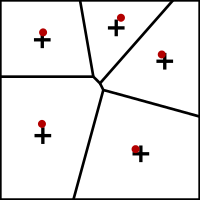
\includegraphics[width=5cm]{lloyd_iterazione_3.png}
\centering
\end{figure}

\paragraph{Iterazione 4}

Ogni drone si trova ora posizionato sopra il centro di massa della propria cella, di conseguenza l'algoritmo ha raggiunto la convergenza.

\begin{figure}[H]
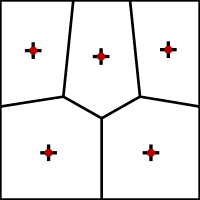
\includegraphics[width=5cm]{lloyd_iterazione_4.png}
\centering
\end{figure}

\section{Concezione intuitiva della convergenza dell'algoritmo}

Intuitivamente, si può dire che l'algoritmo converge in quanto i punti che si trovano a minor distanza tra loro tendono a compiere un movimento più alto, mentre i punti che si trovano a distanze elevate tendono a muoversi meno.

\section{Esecuzione dell'algoritmo}

L'algoritmo, anziché essere eseguito centralmente, viene distribuito tra i centri di calcolo dei vari droni.

L'esecuzione, per ogni drone, diviene quindi:

\begin{enumerate}
	\item Fino al segnale di \textit{STOP}, ripeti:
	\begin{enumerate}
		\item Attendi le coordinate relative alla posizione degli altri droni, comunicate via radio
		\item Ottieni dal \textit{controllo di volo} le proprie coordinate
		\item Esegui la funzione \name{TargetPos}, che restituisce le coordinate del punto da raggiungere (vedi la sezione \ref{TargetPos} per i dettagli)
		\item Comunica l'output al controllo di volo
	\end{enumerate}
\end{enumerate}

\pagebreak

\chapter{Prototipazione}

Al fine di realizzare l'algoritmo, si è reso necessario attraversare una prima fase di prototipazione.

Le specifiche del linguaggio di prototipazione erano le seguenti: un linguaggio dinamico che permettesse una concisa scrittura del codice e una rapida compilazione; strumenti di \textit{testing} integrati per verificare l'effettiva correttezza delle funzioni implementate; la disponibilità di un framework grafico per effettuare simulazioni in modo rapido e dimanico.

La scelta è ricaduta quindi sul linguaggio Python\footnote{https://www.python.org/} e sul framework \textit{Pygame}\footnote{https://www.pygame.org/}

\begin{figure}[H]
\centering

\includegraphics[width=5cm]{python.png}

\includegraphics[width=5cm]{pygame.png}

\end{figure}

\section{Codifica}

Il codice dell'implementazione Python non viene qui riportato, in quanto viene successivamente illustrato e commentato il porting dei prototipi nel linguaggio \textit{OpenModelica}.

È comunque possibile prendere visione del codice di prototipazione presso il repository Github del progetto\footnote{https://github.com/zapateo/Tesi-Gianluca-Mondini-UNIPI}.


\section{Testing}

Al fine di implementare un meccanismo di testing rapido e completo si è optato per il framework \textit{doctest}.

\paragraph{Esempio di testing tramite \textit{doctest}}

Prendiamo, ad esempio, l'implementazione di una funzione triviale \textit{somma} che, dati due numeri $a$ e $b$, restituisca la loro somma.

La libreria \textit{doctest} ci permette di definire, all'interno della documentazione della funzione, alcuni test che fungono inoltre da codice di esempio.

\begin{figure}[H]
\begin{lstlisting}[language=Python]
def somma(a, b):
	"""
	Restituisce la somma di a e b
	
	>>> somma(4, 5)
	9
	
	>>> somma(0, -3)
	-3
	"""
	return a + b
\end{lstlisting}
\end{figure}

È adesso necessario richiamare all'interno \textit{main} del codice sorgente l'esecuzione dei vari test, tramite

\begin{figure}[H]
\begin{lstlisting}[language=Python]
if __name__ == "__main__":
    import doctest
    doctest.testmod()
\end{lstlisting}
\end{figure}

Eseguendo quindi il codice sorgente, verrano eseguiti i test presenti nella documentazione delle varie funzioni e l'output verrà confrontato con quello atteso. Nel caso in cui tutti i test vengano superati non verrà mostrato alcun output a schermo, in caso contrario un messaggio d'errore indicherà il test non superato, l'output atteso e l'output ottenuto.

\pagebreak

\chapter{Implementazione in \textit{OpenModelica}}

L'implementazione dell'algoritmo di Lloyd richiede una funzione che effettui la tassellazione di Voronoi, la quale a sua volta utilizza una serie di funzioni geometriche che operano nello spazio bidimensionale.

Nell'implementazione che verrà illustrata successivamente, si è scelto di implementare in primo luogo l'algoritmo utilizzando il linguaggio Python per avere a disposizione una maggior quantità di strumenti di debugging e testing; successivamente è stato effettuato il porting del codice in \textit{OpenModelica}

\section{OpenModelica}

\begin{figure}[H]
\centering

\includegraphics[scale=0.5]{openmodelica.png}
\end{figure}

\textit{OpenModelica} è un implementazione \textit{open source} del linguaggio di modellazione \textit{Modelica}, che permette la modellazione, simulazione, ottimizzazione e analisi di complessi sistemi dinamici. \textit{OpenModelica} viene utilizzato sia in ambito accademico sia in ambito industriale.

L'ambiente \textit{OpenModelica}, implementato nei linguaggi C e C++, fornisce una serie di strumenti di lavoro, tra cui:

\begin{description}
	\item[omc] compila un file sorgente \textit{OpenModelica} generando la rispettiva \textit{classe}
	\item[OMEdit] software che permette, tra le varie cose, di "connettere" tramite un'interfaccia grafica le varie classi per comporre sistemi complessi
	\item[OMShell] shell interattiva che esegue comandi impartiti singolarmente, utile per effettuare una rapida prototipazione
\end{description}

Per ulteriori informazioni si rimanda al sito ufficiale del progetto\footnote{https://openmodelica.org/} e al documento di specifica Modelica\footnote{https://www.modelica.org/documents/ModelicaSpec34.pdf}

\section{Un approccio funzionale}

Nell'implementazione del codice si è optato per un approccio funzionale. In pratica ogni "modulo" viene implementato tramite una funzione che abbia un determinato dominio di input e codominio di output e viene codificata in modo tale da evitare \textit{effetti collaterali} al di fuori di se stessa. Questo garantisce che, data una funzione e un insieme di input, si possa determinare univocamente l'output, indipendentemente dal valore di parametri esterni alla funzione. Il tutto può essere chiarito con un esempio:

\begin{figure}[H]
\begin{lstlisting}
A = 0
B = 20

func F(C, D) {
	A = A + 10
	return C + D + A
}

output = F(30, 40)
\end{lstlisting}
\caption{Un implementazione non-funzionale di \name{F}}
\end{figure}

La funzione \name{F} restituisce la somma di \name{C}, \name{D} ed \name{A}. In questo caso il valore \name{output} sarà $30 + 40 + 10 = 80$.

La funzione presenta però un problema: eseguendo nuovamente la funzione con gli stessi argomenti, l'output sarà $30 + 40 + 20 = 90$ in quanto il valore di \name{A} è variato, ovvero ha subito un \textit{effetto collaterale} dalla chiamata della funzione.

Inoltre, variando \name{A} al di fuori della funzione il suo output cambierà di conseguenza

\begin{figure}[H]
\begin{lstlisting}
A = 0
B = 20

func F(C, D) {
	A = A + 10
	return C + D + A
}

output = F(30, 40)

A = 100

output = F(30, 40)
\end{lstlisting}
\caption{La stessa funzione \name{F}, chiamata con gli stessi argomenti in momenti diversi, restituisce output diversi}
\end{figure}

Non è quindi possibile stabilire, a priori, l'output della funzione dati gli argomenti se non si conosce anche, per intero, l'ambiente nel quale la funzione viene eseguita.

L'approccio funzionale prevede quindi di implementare la funzione \name{F} nel seguente modo:

\begin{figure}[H]
\begin{lstlisting}
A = 0
B = 20

func F(C, D, A) {
	A = A + 10
	return C + D + A, A
}

output, A = F(30, 40)
\end{lstlisting}
\label{implementazione_funzionale_F}
\caption{Un implementazione funzionale della funzione \name{F}}
\end{figure}

In questo caso la funzione non accetta più 2 argomenti, bensì 3, come era implicitamente codificato nella versione precedente. Si noti inoltre che la funzione non restituisce soltanto un valore di output ma 2, il risultato della somma (assegnato qui a \name{output}) e il nuovo valore di \name{A}, che ha subìto un incremento.

Questo nuovo modello semplifica notevolemente lo sviluppo, in quanto la funzione \name{F} è ora svincolata dall'ambiente che la circonda ed è liberamente eseguibile all'interno di altro codice.

Un altro aspetto da considerare è quello del \textit{testing}; come si vedrà più  avanti nella sezione \ref{testing}, è indispensabile realizzare un meccanismo di testing che garantisca l'effettiva correttezza delle funzioni implementate. A questo riguardo l'approccio funzionale scelto semplifica notevolemente questa fase di sviluppo, in quanto è sufficiente effettuare chiamate singole alle varie funzioni per ottenerne l'output da confrontare con un valore di riferimento.

Nel nostro esempio la funzione \name{F} come mostrata nella figura \ref{implementazione_funzionale_F} chiamata con argomenti costanti restituirà sempre lo stesso valore di output.

\section{Diagramma delle dipendenze}

Viene qui illustrato un diagramma contenenti le varie funzioni dell'implementazione \textit{OpenModelica}. Le frecce $\longrightarrow$ rappresentano una dipendenza; ad esempio $A \longrightarrow B$ indica che $A$ effettua una chiamata a $B$ durante la sua esecuzione, e di conseguenza $A$ \textit{dipende da} $B$.

Sono state omesse le funzioni di supporto al testing e al debugging in quanto non strettamente legate all'implementazione di per sè.

In alto è presente la funzione \name{TargetPos}, la quale dipende da \name{CenterOfMass}, \name{VoronoiCell} e \name{EdgesToVertices}.

In basso troviamo \name{CompareReal}, che dipende esclusivamente da funzioni integrate in \textit{OpenModelica}.

\begin{figure}[H]
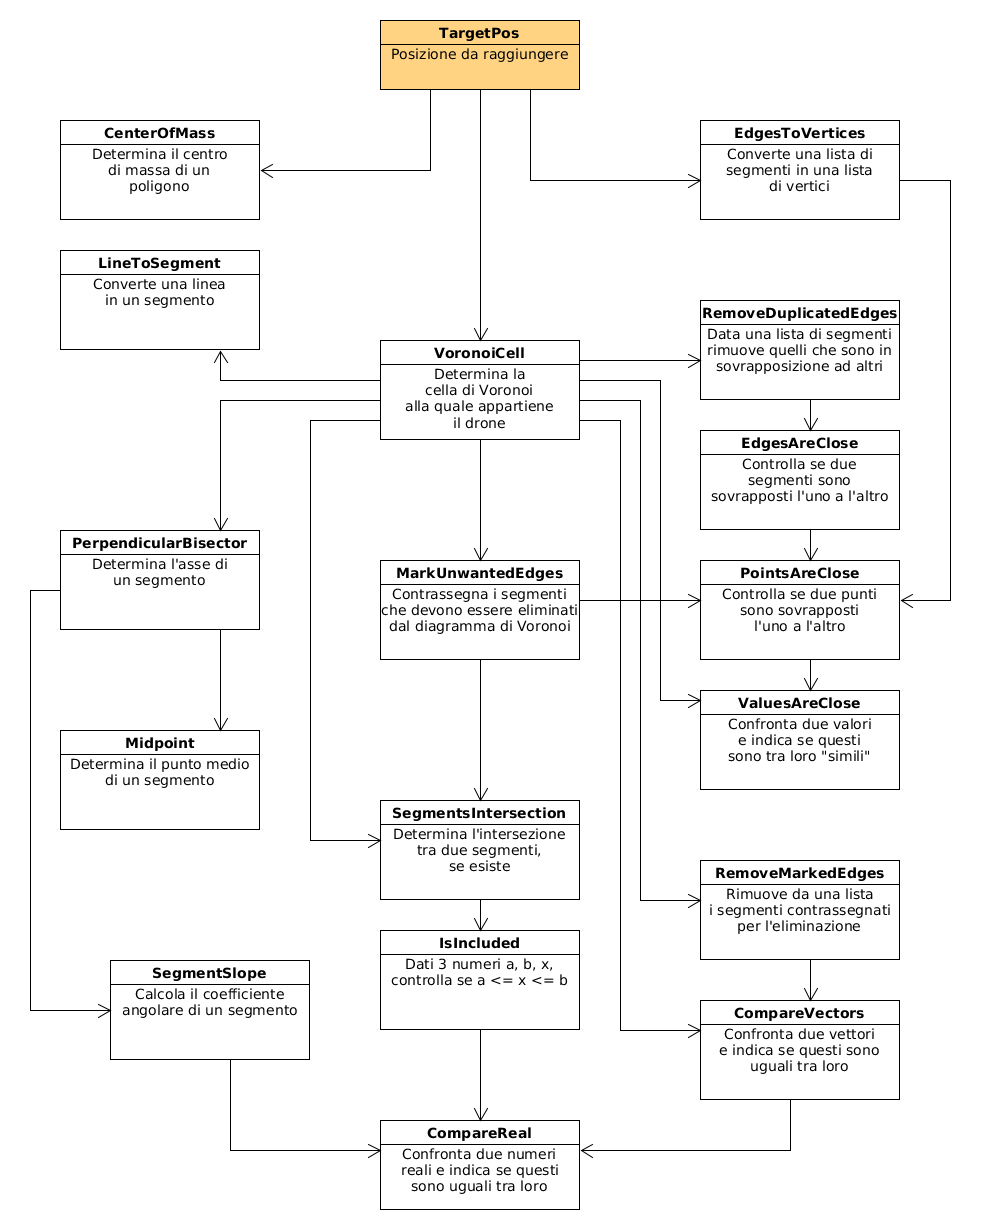
\includegraphics[width=15cm]{uml_diagram/uml_diagram_lloyd.png}
\centering
\caption{Diagramma delle dipendenze delle varie funzioni}
\end{figure}

\section{Scelte implementative}

Come si vedrà in seguito, anzichè definire \textit{tipi} personalizzati si è deciso di ricorrere alle strutture dati già presenti in \textit{OpenModelica}.

Ad esempio, un punto dello spazio può essere rappresentato sia come \textit{record} tramite

\begin{figure}[H]
\begin{lstlisting}[language=Modelica]
record Point
	Real x, y;
end Point;
\end{lstlisting}
\end{figure}

sia come vettore

\begin{lstlisting}[language=Modelica]
Real [2] point;
\end{lstlisting}

La scelta è ricade su quest'ultima implementazione in quanto è possibile utilizzare una serie di funzioni primitive (principalmente per lavorare su liste) già definite in \textit{OpenModelica} che avrebbero richiesto altrimenti richiesto l'implementazione manuale tramite un linguaggio di più basso livello.

I punti a sfavore dell'utilizzo di un vettore al posto di una struttura dati personalizzata sono:

\begin{itemize}
	\item L'impossibilità di accedere ai membri tramite il loro nome bensì tramite l'indice legato alla loro posizione. Ad esempio, per accedere alla coordinata $y$ di un punto non è possibile utilizzare \verb|point.y| ma \verb|point[2]|, perdendo quindi di leggibilità
	\item L'impossibilità di aggiungere ulteriori campi contenenti informazioni. A questo riguardo si veda la sezione \ref{mark_unwanted_edges}
\end{itemize}

\section{Rappresentazione del punto geometrico}

Per poter indicare un punto nello spazio bidimensionale, è necessario definire una struttura dati rappresentante una tupla \textit{x, y}. A questo fine viene utilizzato un vettore bidimensionale definito tramite

\begin{lstlisting}[language=Modelica]
Real [2] point;
\end{lstlisting}

Nel caso in cui debba essere dichiarato un vettore di punti, si dichiara una matrice tramite

\begin{lstlisting}[language=Modelica]
Real [:, 2] some_points;
\end{lstlisting}

Il carattere \verb|:| posto in prima posizione tra le parentesi quadre indica che la prima dimensione della matrice \verb|some_points| non è conosciuta a priori.

\section{Verifica della sovrapposizione di due punti}

Può verificarsi che, in seguito a ..., ci si trovi nella situazione in cui due punti sovrapposti non superino il test di equalità. Ad esempio:
\[
P_1 = (4.0, 2.0)
\]
\[
P_2 = (4.00001, 1.999999)
\]

I punti $P_1$ e $P_2$, pur potendo essere considerati sovrapposti in relazione allo spazio metrico in cui si trovano, sono considerati diversi da loro per via di errori di approssimazione del calcolatore.

% TODO riscrivere la funzione points are close in stile EdgesAreClose

Si è quindi implementata una funzione che discrimini i punti diversi tra loro da quelli "apparentemente diversi", ovvero una funzione che verifichi se due punti sono tra loro \textit{vicini}.

\begin{figure}[H]
\modelicaclass{PointsAreClose.mo}
\end{figure}

\section{Rappresentazione del segmento geometrico}

Per rappresentare un segmento, si considera un vettore di 4 elementi, nella forma

\[
(x_0, y_0, x_1, y_1)
\]

dove $(x_0, y_0)$ è il punto iniziale del segmento e $(x_1, y_1)$ è il punto finale.

\begin{figure}[H]
\centering
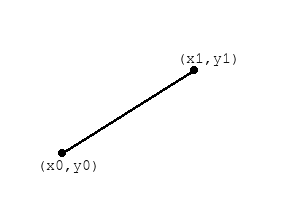
\includegraphics[scale=0.5]{segmento.png}
\end{figure}

Questo si traduce, in ambiente \textit{OpenModelica}, in:

\begin{lstlisting}[language=Modelica]
Real [4] edge;

edge[1] := x_1;
edge[2] := y_1;
edge[3] := x_2;
edge[4] := y_2;
\end{lstlisting}

\section{Verifica della sovrapposizione di due segmenti}

La verifica della sovrapposizione di due segmenti viene effettuata in modo analogo a quella della sovrapposizione di due punti, e fa uso proprio di quest'ultima funzione.

Formalmente, due segmenti sono considerati sovrapposti se il punto iniziale del primo si sovrappone al punto iniziale del secondo e contemporaneamente il punto finale del primo si sovrappone al punto finale del secondo.

\begin{figure}[H]
\modelicaclass{EdgesAreClose.mo}
\end{figure}

\section{Linea}

Una \textit{linea} è matematicamente identificata da una tupla di 3 elementi $a$, $b$ e $c$ tali che

\[
a x + b y + c = 0
\]

In \textit{OpenModelica}, si rappresenterà quindi come un vettore di 3 elementi
\begin{lstlisting}[language=Modelica]
Real [3] line;

line[1] := a;
line[2] := b;
line[3] := c;
\end{lstlisting}

\section{Conversione da linea a segmento}

Può essere necessario convertire una linea, priva di un punto di inizio e fine, in un segmento, ben delimitato. Per fare ciò è stata implementata la funzione

\[
	\text{LineToSegment} : R[3] \longrightarrow R[4]
\]

\modelicaclass{LineToSegment.mo}

\section{Intersezione tra segmenti}

Una delle funzioni principalmente utilizzate dall'algoritmo di tassellazione di Voronoi è quella responsabile di determinare l'eventuale punto di intersezione tra due segmenti.

È necessario notare che, avendo a che fare con segmenti di lunghezza finita e non con delle rette, è possibile che due segmenti non si intersechino tra loro pur non essendo paralleli.

\begin{figure}[H]
\centering
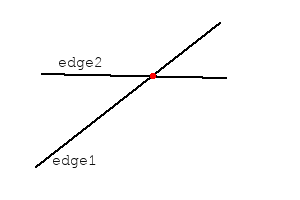
\includegraphics[scale=0.5]{intersection.png}
\end{figure}

L'algoritmo implementato è il seguente \footnote{Il codice è un adattamento di https://www.cs.hmc.edu/ACM/lectures/intersections.html}

\modelicaclass{SegmentsIntersection.mo}

Oltre a restituire un vettore bidimensionale \verb|intersection| viene anche restituito un booleano \verb|valid|, che sta ad indicare se il valore contenuto in \verb|intersection| è valido o meno.

\section{Asse di un segmento}

La funzione \name{VoronoiCell} fa ampio uso della funzione \name{PerpendicularBisector}, che restituisce l'asse del segmento passato come argomento.

\[
\text{PerpendicularBisector} : \text{Segmento} \longrightarrow \text{Linea}
\]


Vengono discriminati i 3 casi in cui:

\begin{itemize}
	\item Il segmento sia verticale; in tal caso l'asse sarà orizzontale;
	\item Il segmento sia orizzontale; in tal caso l'asse sarà verticale;
	\item Il segmento non sia nè verticale nè orizzontale: caso più frequente
\end{itemize}

\begin{figure}[H]
\centering
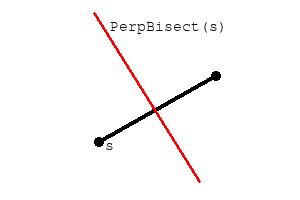
\includegraphics[scale=0.7]{PerpendicularBisector.png}
\end{figure}

\modelicaclass{PerpendicularBisector.mo}

\section{Centro di massa}

Al fine di implementare l'algoritmo di Lloyd è necessario definire una funzione che, presa in ingresso una lista di vertici, ne calcoli il centro di massa.

Dato un poligono di $n$ vertici $(x_0, y_0), (x_1, y_1), ..(x_{n-1},y_{n-1})$ il centro di massa ha coordinate $(C_X, C_Y)$ definite come

\[
C_x = \frac{1}{6 A} \sum_{i=0}^{n-1} (x_i + x_{i+1}) (x_i y_{i+1} - x_{i+1} y_i)
\]

\[
C_y = \frac{1}{6 A} \sum_{i=0}^{n-1} (y_i + y_{i+1}) (x_i y_{i+1} - x_{i+1} y_i)
\]

dove $A$ è l'area del poligono \textit{con segno}

\[
A = \frac{1}{2} \sum_{i=0}^{n-1} (x_i y_{i+1} - x_{i+1} y_i)
\]

\begin{figure}[H]
\centering
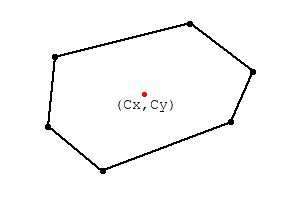
\includegraphics[scale=0.6]{CenterOfMass.png}
\caption{Il punto $p$ viene restituito dalla chiamata a \name{CenterOfMass} che ha come argomento la lista delle coordinate dei vari vertici del poligono}
\end{figure}

Ne deriva quindi la seguente codifica:

\modelicaclass{CenterOfMass.mo}

\section{Ricerca ed eliminazione dei segmenti in eccesso}

Durante l'esecuzione dell'algoritmo di Voronoi si presenta la necessità di rimuovere dei segmenti che non fanno più parte del diagramma. Si presenta il problema di come effettuare questa operazione senza arrecare danno all'iterazione in corso proprio sulla lista dalla quale vanno rimossi gli elementi.

Inoltre, come precedentemente detto, non è possibile aggiungere un campo ad ogni segmento indicando l'effettiva necessità di eliminazione.

La scelta cade quindi sull'assegnare il valore $-1$ ad ogni componente del segmento, considerandolo quindi un segmento nullo, da eliminare.

\begin{lstlisting}[language=Modelica]
edge := {-1, -1, -1, -1};
\end{lstlisting}

Successivamente, utilizzando la funzione \verb|CompareVector| si controlla se il segmento è contrassegnato per l'eliminazione

\begin{figure}[H]
\begin{lstlisting}
if CompareVector(edge, {-1, -1, -1, -1}) then
	// Considera 'edge' come un segmento da eliminare
else
	// Considera 'edge' come un segmento valido
end if;
\end{lstlisting}
\end{figure}

La funzione \verb|MarkUnwantedEdges| contrassegna tutti i segmenti che devono essere rimossi dalla lista di segmenti. In particolare, se un segmento si trova dietro ad un altro quello "nascosto" deve essere eliminato in quanto non può più far parte dell'insieme.

\label{mark_unwanted_edges}

\begin{figure}[H]
\centering
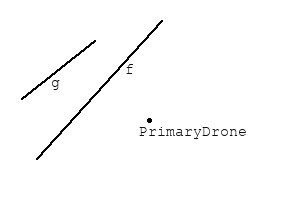
\includegraphics[scale=0.7]{rimozione_segmento.png}
\caption{Esempio nel quale il segmento $g$ deve essere rimosso, in quanto il segmento $f$ si pone tra esso e il \textit{PrimaryDrone}. La funzione \name{MarkUnwantedEdges} contrassegnerà $g$ per l'eliminazione, mentre \name{RemoveMarkedEdges} lo cancellerà definitivamente.}
\end{figure}

\begin{figure}[H]
\centering
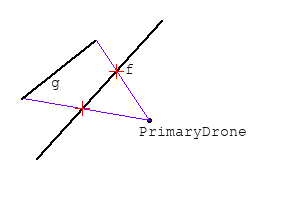
\includegraphics[scale=0.7]{rimozione_segmento2.png}
\caption{I segmenti di unione tra \name{PrimaryDrone} e gli estremi di $g$ collidono con il segmento $f$; questo fa sì che $g$ venga contrassegnato per l'eliminazione.}
\end{figure}

\modelicaclass{MarkUnwantedEdges.mo}

La funzione \verb|RemoveMarkedEdges| restituisce una lista di segmenti dalla quale sono stati rimossi tutti i segmenti contrassegnati per l'eliminazione.

\modelicaclass{RemoveMarkedEdges.mo}

\section{La funzione \name{VoronoiCell}}

Come precedentemente detto, l'algoritmo di Lloyd è implementato tramite iterazioni successive dell'algoritmo di Voronoi.

La funzione \name{VoronoiCell} restituisce esclusivamente la cella di appartenenza di un drone specificato, anziché la tassellazione dell'intera area; considerato che l'algoritmo è distribuito ogni drone necessita di conoscere esclusivamente la propria posizione \textit{target}, e soltanto la posizione attuale dei restanti droni.

L'idea è quindi quella di implementare la seguente funzione:

\[
\text{VoronoiCell} : (\text{drone stesso}, \text{altri droni}, \text{bordi}) \longrightarrow \text{cella drone stesso}
\]

I passaggi fondamentali dell'algoritmo implementato sono i seguenti:

%TODO mancano alcuni passaggi
%TODO correggere maiuscole/minuscole

\begin{enumerate}
	\item Per ogni \name{drone} contenuto in \name{other drones} (ovvero la lista degli altri droni)
	\begin{enumerate}
		\item viene creato un segmento \name{union edge} che unisce il drone stesso (\name{primary drone}) con \name{drone}
		\item viene determinato l'asse di \name{union edge}, che prende il nome di \name{perp bisect}
		\item viene inizializzata una lista vuota \name{intersections} che andrà a contenere i punti di intersezione trovati
		\item Per ogni bordo \name{edge} contenuto in \name{edges}
		\begin{enumerate}
			\item viene cercato l'eventuale punto di intersezione tra \name{perp bisect} ed \name{edge}
			\item se il punto di intersezione esiste
			\begin{enumerate}
				\item contrassegno \name{edge} per la cancellazione, in quanto verrà sostituito da un nuovo bordo
				\item determino quale estremo di \name{edge} conservare per la creazione del nuovo bordo
				\item aggiunto il punto di intersezione trovato alla lista \name{intersections}
			\end{enumerate}
		\end{enumerate}
		\item se \name{intersections} contiene 2 punti, creo un nuovo bordo che abbia come estremi i 2 punti
	\end{enumerate}
	\item tolgo da \name{edges} i bordi duplicati e quelli contrassegnati per l'eliminazione
\end{enumerate}

\subsection{Esempio grafico di applicazione dell'algoritmo di Voronoi}

Vediamo adesso l'applicazione dell'algoritmo di Voronoi alla seguente situazione: l'area è delimitata da un poligono a 5 lati; in rosso è visibile quello che viene chiamato \name{PrimaryDrone}, ovvero il drone che effettua la chiamata a \name{VoronoiCell} e per il quale si intende calcolare la cella associata; i restanti 2 puntini neri rappresentano gli altri due droni.

\begin{figure}[H]
\centering
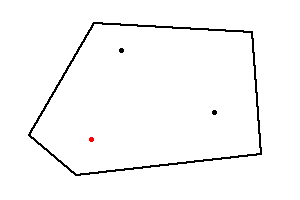
\includegraphics[scale=0.7]{voronoi1.png}
\end{figure}

Si determina quindi il segmento che unisce \name{PrimaryDrone} con uno degli altri droni, in questo caso quello più in alto; si traccia l'asse del segmento trovato e si determinano i punti di intersezione con i bordi dell'area, che nella figura sono contrassegnati da croci rosse.

\begin{figure}[H]
\centering
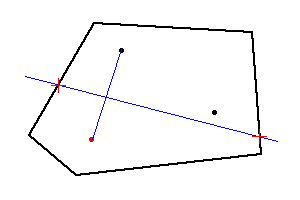
\includegraphics[scale=0.7]{voronoi2.png}
\end{figure}

Si crea un nuovo bordo che unisce i due punti di intersezione. Tutti i segmenti che si trovino "dietro" (si veda la sezione \ref{mark_unwanted_edges}) al nuovo segmento vengono contrassegnati per l'eliminazione.

Si noti inoltre che i due bordi con i quali l'asse intersecava sono stati sostituiti da due nuovi bordi, di lunghezza inferiore.

\begin{figure}[H]
\centering
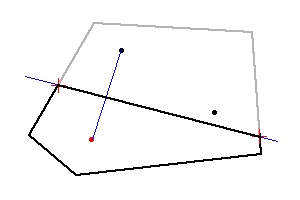
\includegraphics[scale=0.7]{voronoi3.png}
\end{figure}

Si ripete il procedimento anche per l'altro drone, ed essendo in questo caso i droni totali in numero pari a 3 si conclude l'algoritmo.

Il poligono contornato in nero è quindi la cella di Voronoi associata al \name{PrimaryDrone}

\begin{figure}[H]
\centering
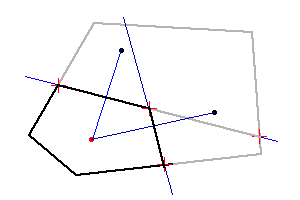
\includegraphics[scale=0.7]{voronoi4.png}
\end{figure}

Il codice che ne deriva è il seguente:

\modelicaclass{VoronoiCell.mo}

\section{La funzione \name{TargetPos}}

\label{TargetPos}

La funzione \name{TargetPos} effettua una singola iterazione dell'algoritmo di Lloyd, ovvero:

\begin{enumerate}
	\item \label{TargetPos_step1} Determina la cella di Voronoi relativa al drone stesso
	\item Calcola il centro di massa della cella determinata al punto \ref{TargetPos_step1}
\end{enumerate}

% note sulla chiamata più volte nel tempo che consente la convergenza

\begin{figure}[H]
\modelicaclass{TargetPos.mo}
\end{figure}

\section{Testing del codice}

\label{testing}

Attualmente \textit{OpenModelica} non fornisce un meccanismo di testing solido e standardizzato. Per questo motivo è stato necessario realizzare un sistema che automatizzasse la verifica della correttezza delle funzioni implementate.

A questo proposito si è deciso di ricorrere ad uno script Python che:

\begin{enumerate}
	\item Ottenga la lista delle classi implementate
	\item Ottenga la lista dei test da effettuare
	\item Compili le classi
	\item Crei un file contenente le istruzioni per eseguire tutti i test
	\item Esegua, uno dopo l'altro, i vari test
	\item Restituisca a schermo un output indicante l'esito dei vari test
\end{enumerate}

\lstinputlisting[language=Python]{../Implementazioni algoritmo/openmodelica/runtests}

\pagebreak

\chapter{Conclusioni}

\chapter*{Bibliografia}

\begin{itemize}
	\item https://en.wikipedia.org/wiki/Lloyd\%27s\_algorithm
	\item github.com/zapateocallisto
	\item https://en.wikipedia.org/wiki/Centroid
\end{itemize}

\end{document}